\documentclass[convert]{standalone}

\usepackage{tikz}
\usepackage{graphicx}
\pagestyle{empty}

% INT_AY20_MP3_L22_Fig06_F_mag_dir.tex

\begin{document}
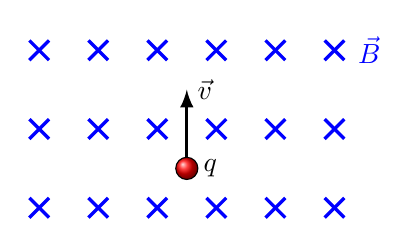
\begin{tikzpicture}

	% Magnetic field indicators with label node
	
	\def\delta{0.125}		% Size of x's for magnetic field
	
	\foreach \x in {-1.875, -1.125, ..., 1.875}
	\foreach \y in {-1, 0, 1}
		{
		\begin{scope}[very thick, blue]
		
			\draw (\x + \delta, \y + \delta) -- (\x - \delta, \y - \delta);
			\draw (\x + \delta, \y - \delta) -- (\x - \delta, \y + \delta);
			
		\end{scope}
		}
		
	\node at (1.875, 1) [right = 0.5 em, blue] {${\vec B}$};
		
	% Positive charge with velocity vector
	
	\draw [->, > = latex, very thick] (0, -0.5) -- (0, 0.5) node [right] {${\vec v}$};
	\draw [ball color = red] (0, -0.5) circle (4 pt) node [right = 0.25 em] {$q$};

\end{tikzpicture}
\end{document}